\documentclass[12pt]{report}
\usepackage{scribe,graphicx,graphics}
\usepackage{float}
\usepackage{siunitx}
\course{CSE 389D} 	
\coursetitle{Mathematical Modeling}	
\semester{Spring 2025}
\lecturer{} % Due Date: {\bf Mon, Oct 3 2016}}
\lecturetitle{Problem Set}
\lecturenumber{2}   
\lecturedate{}    
\usepackage{enumerate}
\newcommand{\remind}[1]{\textcolor{red}{\textbf{#1}}} %To remind me of unfinished work to fix later
\newcommand{\hide}[1]{} %To hide large blocks of code without using % symbols

\newcommand{\ep}{\varepsilon}
\newcommand{\vp}{\varphi}
\newcommand{\lam}{\lambda}
\newcommand{\Lam}{\Lambda}
%\newcommand{\abs}[1]{\ensuremath{\left\lvert#1\right\rvert}} % This clashes with the physics package
%\newcommand{\norm}[1]{\ensuremath{\left\lVert#1\right\rVert}} % This clashes with the physics package
\newcommand{\floor}[1]{\ensuremath{\left\lfloor#1\right\rfloor}}
\newcommand{\ceil}[1]{\ensuremath{\left\lceil#1\right\rceil}}
\newcommand{\A}{\mathbb{A}}
\newcommand{\B}{\mathbb{B}}
\newcommand{\C}{\mathbb{C}}
\newcommand{\D}{\mathbb{D}}
\newcommand{\E}{\mathbb{E}}
\newcommand{\F}{\mathbb{F}}
\newcommand{\K}{\mathbb{K}}
\newcommand{\N}{\mathbb{N}}
\newcommand{\Q}{\mathbb{Q}}
\newcommand{\R}{\mathbb{R}}
\newcommand{\T}{\mathbb{T}}
\newcommand{\X}{\mathbb{X}}
\newcommand{\Y}{\mathbb{Y}}
\newcommand{\Z}{\mathbb{Z}}
\newcommand{\As}{\mathcal{A}}
\newcommand{\Bs}{\mathcal{B}}
\newcommand{\Cs}{\mathcal{C}}
\newcommand{\Ds}{\mathcal{D}}
\newcommand{\Es}{\mathcal{E}}
\newcommand{\Fs}{\mathcal{F}}
\newcommand{\Gs}{\mathcal{G}}
\newcommand{\Hs}{\mathcal{H}}
\newcommand{\Is}{\mathcal{I}}
\newcommand{\Js}{\mathcal{J}}
\newcommand{\Ks}{\mathcal{K}}
\newcommand{\Ls}{\mathcal{L}}
\newcommand{\Ms}{\mathcal{M}}
\newcommand{\Ns}{\mathcal{N}}
\newcommand{\Os}{\mathcal{O}}
\newcommand{\Ps}{\mathcal{P}}
\newcommand{\Qs}{\mathcal{Q}}
\newcommand{\Rs}{\mathcal{R}}
\newcommand{\Ss}{\mathcal{S}}
\newcommand{\Ts}{\mathcal{T}}
\newcommand{\Us}{\mathcal{U}}
\newcommand{\Vs}{\mathcal{V}}
\newcommand{\Ws}{\mathcal{W}}
\newcommand{\Xs}{\mathcal{X}}
\newcommand{\Ys}{\mathcal{Y}}
\newcommand{\Zs}{\mathcal{Z}}
\newcommand{\ab}{\textbf{a}}
\newcommand{\bb}{\textbf{b}}
\newcommand{\cb}{\textbf{c}}
\newcommand{\db}{\textbf{d}}
\newcommand{\ub}{\textbf{u}}
\newcommand{\sbb}{\textbf{s}}
%\renewcommand{\vb}{\textbf{v}} % This clashes with the physics package (the physics package already defines the \vb command)
\newcommand{\wb}{\textbf{w}}
\newcommand{\xb}{\textbf{x}}
\newcommand{\yb}{\textbf{y}}
\newcommand{\zb}{\textbf{z}}
\newcommand{\vbb}{\textbf{v}}
\newcommand{\Ab}{\textbf{A}}
\newcommand{\Bb}{\textbf{B}}
\newcommand{\Cb}{\textbf{C}}
\newcommand{\Db}{\textbf{D}}
\newcommand{\eb}{\textbf{e}}
\newcommand{\ex}{\textbf{e}_x}
\newcommand{\ey}{\textbf{e}_y}
\newcommand{\ez}{\textbf{e}_z}
\newcommand{\zerob}{\mathbf{0}}
\newcommand{\abar}{\overline{a}}
\newcommand{\bbar}{\overline{b}}
\newcommand{\cbar}{\overline{c}}
\newcommand{\dbar}{\overline{d}}
\newcommand{\ubar}{\overline{u}}
\newcommand{\vbar}{\overline{v}}
\newcommand{\wbar}{\overline{w}}
\newcommand{\xbar}{\overline{x}}
\newcommand{\ybar}{\overline{y}}
\newcommand{\zbar}{\overline{z}}
\newcommand{\Abar}{\overline{A}}
\newcommand{\Bbar}{\overline{B}}
\newcommand{\Cbar}{\overline{C}}
\newcommand{\Dbar}{\overline{D}}
\newcommand{\Ubar}{\overline{U}}
\newcommand{\Vbar}{\overline{V}}
\newcommand{\Wbar}{\overline{W}}
\newcommand{\Xbar}{\overline{X}}
\newcommand{\Ybar}{\overline{Y}}
\newcommand{\Zbar}{\overline{Z}}
\newcommand{\Aint}{A^\circ}
\newcommand{\Bint}{B^\circ}
\newcommand{\limk}{\lim_{k\to\infty}}
\newcommand{\limm}{\lim_{m\to\infty}}
\newcommand{\limn}{\lim_{n\to\infty}}
\newcommand{\limx}[1][a]{\lim_{x\to#1}}
\newcommand{\liminfm}{\liminf_{m\to\infty}}
\newcommand{\limsupm}{\limsup_{m\to\infty}}
\newcommand{\liminfn}{\liminf_{n\to\infty}}
\newcommand{\limsupn}{\limsup_{n\to\infty}}
\newcommand{\sumkn}{\sum_{k=1}^n}
\newcommand{\sumk}[1][1]{\sum_{k=#1}^\infty}
\newcommand{\summ}[1][1]{\sum_{m=#1}^\infty}
\newcommand{\sumn}[1][1]{\sum_{n=#1}^\infty}
\newcommand{\emp}{\varnothing}
\newcommand{\exc}{\backslash}
\newcommand{\sub}{\subseteq}
\newcommand{\sups}{\supseteq}
\newcommand{\capp}{\bigcap}
\newcommand{\cupp}{\bigcup}
\newcommand{\kupp}{\bigsqcup}
\newcommand{\cappkn}{\bigcap_{k=1}^n}
\newcommand{\cuppkn}{\bigcup_{k=1}^n}
\newcommand{\kuppkn}{\bigsqcup_{k=1}^n}
\newcommand{\cappk}[1][1]{\bigcap_{k=#1}^\infty}
\newcommand{\cuppk}[1][1]{\bigcup_{k=#1}^\infty}
\newcommand{\cappm}[1][1]{\bigcap_{m=#1}^\infty}
\newcommand{\cuppm}[1][1]{\bigcup_{m=#1}^\infty}
\newcommand{\cappn}[1][1]{\bigcap_{n=#1}^\infty}
\newcommand{\cuppn}[1][1]{\bigcup_{n=#1}^\infty}
\newcommand{\kuppk}[1][1]{\bigsqcup_{k=#1}^\infty}
\newcommand{\kuppm}[1][1]{\bigsqcup_{m=#1}^\infty}
\newcommand{\kuppn}[1][1]{\bigsqcup_{n=#1}^\infty}
\newcommand{\cappa}{\bigcap_{\alpha\in I}}
\newcommand{\cuppa}{\bigcup_{\alpha\in I}}
\newcommand{\kuppa}{\bigsqcup_{\alpha\in I}}
\newcommand{\Rx}{\overline{\mathbb{R}}}
\newcommand{\dx}{\,dx}
\newcommand{\dy}{\,dy}
\newcommand{\dt}{\,dt}
\newcommand{\dax}{\,d\alpha(x)}
\newcommand{\dbx}{\,d\beta(x)}
\DeclareMathOperator{\glb}{\text{glb}}
\DeclareMathOperator{\lub}{\text{lub}}
\newcommand{\xh}{\widehat{x}}
\newcommand{\yh}{\widehat{y}}
\newcommand{\zh}{\widehat{z}}
\newcommand{\<}{\langle}
\renewcommand{\>}{\rangle}
\renewcommand{\iff}{\Leftrightarrow}
\DeclareMathOperator{\im}{\text{im}}
\let\spn\relax\let\Re\relax\let\Im\relax
\DeclareMathOperator{\spn}{\text{span}}
\DeclareMathOperator{\sym}{\text{Sym}}
\DeclareMathOperator{\myskew}{\text{Skew}}
\DeclareMathOperator{\Re}{\text{Re}}
\DeclareMathOperator{\Im}{\text{Im}}
\DeclareMathOperator{\diag}{\text{diag}}
\endinput

\theoremheaderfont{\itshape}
\theorembodyfont{\upshape}
\newtheorem{case}{Case}

% Insert your name here!
\scribe{Student Name: Noah Reef}
\newcommand{\rb}{\bold{r}}

\begin{document}
\maketitle
\section*{Problem 2.1}
\subsection*{Part a}
\begin{figure}[H]
    \centering
    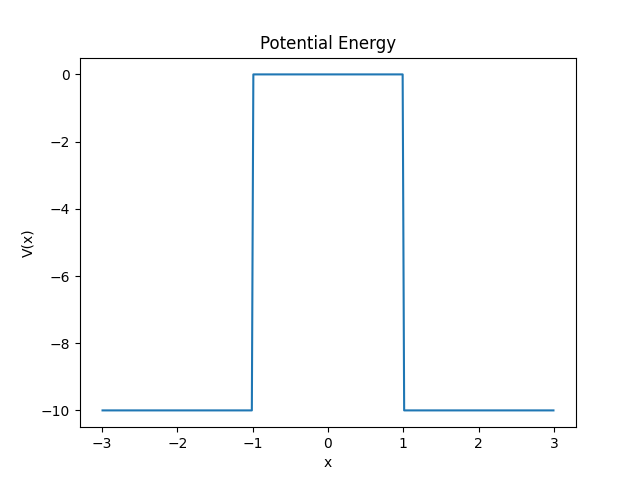
\includegraphics[scale=0.7]{CSE_389D/ps_2/Figure_1.png}
    \caption{Sketch of $V(x)$ for $a=1$,$b=3$, and $V_0 = 10$}
    \label{fig:enter-label}
\end{figure}
The time-independent Schrodinger's equation is given by
\begin{equation*}
    -\frac{\hbar^2}{2m} \frac{d^2\phi(x)}{dx^2} + V(x) \phi(x) = E\phi(x)
\end{equation*}

\subsection*{Part b}
If we consider the bounded state where $-V_0 < E < 0$, and $0 < x < a$, then we get that $V(x) = 0$ and
\begin{equation*}
    -\frac{\hbar^2}{2m} \phi''(x) = E \phi(x) \implies \phi''(x) = \frac{2m |E|}{\hbar^2} \phi(x)
\end{equation*}
solving the differential equation above gives the general solution,
\begin{equation*}
    \phi(x) = Ae^{\kappa x} + Be^{-\kappa x}
\end{equation*}
where
\begin{equation*}
    \kappa = \sqrt{\frac{2m |E|}{\hbar^2}}
\end{equation*}
however since it is symmetric we get that
\begin{equation*}
     \phi(x) = Ae^{\kappa x} + Ae^{-\kappa x} = 2A\cosh(\kappa x)
\end{equation*}
now if we consider the case where $a \leq x \leq b$, we have that $V(x) - V_0$ and get
\begin{equation*}
    -\frac{\hbar^2}{2m}\phi''(x) - V_0 \phi(x) = E\phi(x) \implies \phi''(x) = -\frac{2m(E + V_0)}{\hbar^2} \phi(x)
\end{equation*}
solving the above differential equation yields the following general solution
\begin{equation*}
    \phi(x) = C \cos(\xi (b-x)) + D \sin(\xi(b-x))
\end{equation*}
where 
\begin{equation*}
    \xi = \sqrt{\frac{2m(E + V_0)}{\hbar^2}}
\end{equation*}
then since $V(b) = \infty$ we require that $\phi(b) = 0$ and hence 
\begin{equation*}
    \phi(x) = D \sin(\xi (b-x))
\end{equation*}
now $x = a$ we have that
\begin{equation*}
    2A \cosh(\kappa a) = D \sin(\xi(b-a))
\end{equation*}
taking the derivatives 
\begin{equation*}
    2A\kappa \sinh(\kappa a) =  -D\xi\cos(\xi(b-a))
\end{equation*}
then dividing both equations yields
\begin{equation*}
    \frac{\kappa \sinh(\kappa a)}{\cosh(\kappa a)} = -\frac{\xi \cos(\xi(b-a))}{\sin(\xi(b-a))} \implies \kappa \tanh(\kappa a) = -\xi \cot(\xi (b-a)) = -\xi \frac{1 + \tan(\xi a)\tan(\xi b)}{\tan(\xi b) - \tan(\xi a)}
\end{equation*}
thus
\begin{equation*}
\kappa \tanh(\kappa a) + \xi \frac{1 + \tan(\xi a)\tan(\xi b)}{\tan(\xi b) - \tan(\xi a)} = 0
\end{equation*}
letting $v = \xi b$ and $a = \gamma b$ then we get that
\begin{equation*}
    \kappa \tanh(\kappa a) + (v/b) \frac{1 + \tan(\gamma v)\tan(v)}{\tan(v) - \tan(\gamma v)} = 0
\end{equation*}
note that if we define
\begin{equation*}
    S = \frac{b\sqrt{2mV_0}}{\hbar}
\end{equation*}
then we have that
\begin{align*}
    \kappa = \sqrt{\frac{2m|E|}{\hbar^2}} =\sqrt{\frac{2m(V_0 - (E + V_0)}{\hbar^2}} &= \sqrt{\frac{2mV_0}{\hbar^2} -\xi^2} \\
    &= \sqrt{\frac{2mV_0}{\hbar^2} -\frac{v^2}{b^2}} \\
    &= \frac{1}{b} \sqrt{S^2 - v^2}
\end{align*}
therefore we have that
\begin{equation*}
   \sqrt{S^2 - v^2} \tanh(\gamma \sqrt{S^2 - v^2}) - v \frac{1 + \tan(\gamma v)\tan(v)}{\tan(\gamma v) - \tan(v)} = 0
\end{equation*}
and hence our eigenvalues are given by
\begin{equation*}
    E + V_0 = \frac{\hbar^2 \xi^2}{2m} = \frac{\hbar^2 v^2}{2mb^2} \implies \frac{E}{V_0} = -1 + \frac{v^2}{S^2}
\end{equation*}
\subsection*{Part c}
Solving for $v$ from the equation below we get
\begin{align*}
    v_1 &= 9.87725 \\
    v_2 &= 6.84406 \\
    v_3 &= 3.46525 
\end{align*}
plugging these values into the equation
\begin{equation*}
    \frac{E}{V_0} = -1 + \frac{v^2}{S^2} 
\end{equation*}
yields
\begin{align*}
     \frac{E}{V_0} &= -1 + \frac{(9.87725)^2}{S^2} \approx -0.0244\\
      \frac{E}{V_0} &= -1 + \frac{(6.84406)^2}{S^2} \approx -0.5316\\
       \frac{E}{V_0} &= -1 + \frac{(3.46525)^2}{S^2} \approx -0.8799
\end{align*}
as the eigenvalues of the even bounded state problem.
\end{document}
